\subsubsection{Kürzester Weg finden}

Da es nur 8 Knoten im Graph gibt, wurde von Anfang an vermutet, dass die Geschwindigkeit des Algorithmus vernachlässigt werden kann.

Um zu überprüfen, dass diese These stimmt, wurde ein traditioneller Dijkstra Algorithmus in Python implementiert. Dabei wurde von einem Knoten den kürzesten Weg zu allen anderen Knoten im vorgegebenen Graphen berechnet. währenddessen wurde die Zeit für die Berechnungen gestoppt. Um Hardware Einflüsse zu minimieren, wurde dieses Skript auch auf einem Single-Board Computer, namentlich einem Raspberry Pi 4 (4GB) ausgeführt, und einige male wiederholt. Was uns zu nachfolgender Ausgabe und Kenntnissen bringt:

\begin{figure}[H]
\begin{subfigure}{0.275\textwidth}
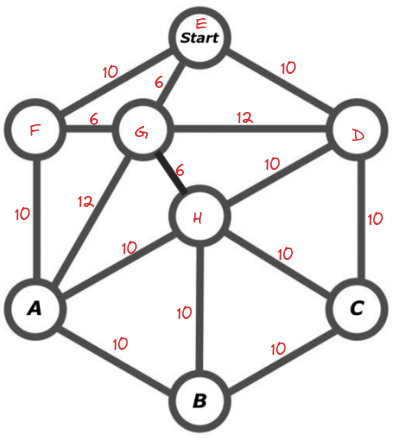
\includegraphics[width=0.95\linewidth]{img/graph_with_weighted_edges.png} 
\caption{Gewichteter Graph}
\label{fig:weighted-graph}
\end{subfigure}
\begin{subfigure}{0.720\textwidth}
\begin{footnotesize}
\begin{verbatim}
Shortest distance from E to A is 18 via path: E -> G -> A
Shortest distance from E to B is 22 via path: E -> G -> H -> B
Shortest distance from E to C is 20 via path: E -> D -> C
Shortest distance from E to D is 10 via path: E -> D
Shortest distance from E to E is 0 via path: E
Shortest distance from E to F is 10 via path: E -> F
Shortest distance from E to G is 6 via path: E -> G
Shortest distance from E to H is 12 via path: E -> G -> H
This calculation took about 0.128ms
\end{verbatim}
\end{footnotesize}
\caption{Skript Ausgabe}
\label{fig:djikstra-test-skript-output}
\end{subfigure}

\caption{Djikstra Algoritmus Test mit Python}
\label{fig:djikstra-test-output}
\end{figure}

Um den kürzesten Pfad achtmal zu berechnen, wurden etwa 0,128 ms benötigt, was ausreichend schnell ist. Aufgrund dieses Tests wurde entschieden, einen selbst implementierten, einfachen Dijkstra-Algorithmus zu verwenden, da es wichtig ist, dass der Algorithmus möglichst leichtgewichtig ist, da nur begrenzte Rechenleistung und Speicher zur Verfügung stehen.

Das Skript wurde in einem Github Gist veröffentlicht und ist unter folgendem Link aufrufbar: \url{https://gist.github.com/dimschlukas/2632116f913b1e10eea9be40e62b2630}

\subsubsection{Winkelerkennung}\label{winkelerkennung}

PLACEHOLDER
Winkel messunge, Bildverzerrung, Tests wieso 20cm abstand

Wie Winkel intern abspeichern, wie mapping, ...

Offset 180 Grad


Hardcoded Winkel, simuliere gemessene Winkel und reageire, Mapping und speichern

\subsubsection{Bilderkennung}

\textbf{Spiegelung}

Starke Spiegelungen stellen ein grosses Problem bei der Erkennung von Knoten dar. Um die Bilder zu entspiegeln, können die Lichtverhältnisse angepasst, Polfilter verwendet oder Nachbearbeitungen durchgeführt werden.\cite{avoid-reflection}

Beleuchtung

\textbf{YOLOv11}

Auf Roboflow\footnote{https://roboflow.com/} Bilder labeled: (Als erstes mit Linie versucht, das geht nicht ev Bild) 

TODO BILD

Mihilfe eines Jupyter skripts Yolo Model trainieren mit 10 Epochs, Confusion Matrix und Bilder:

\begin{figure}[H]
\centering
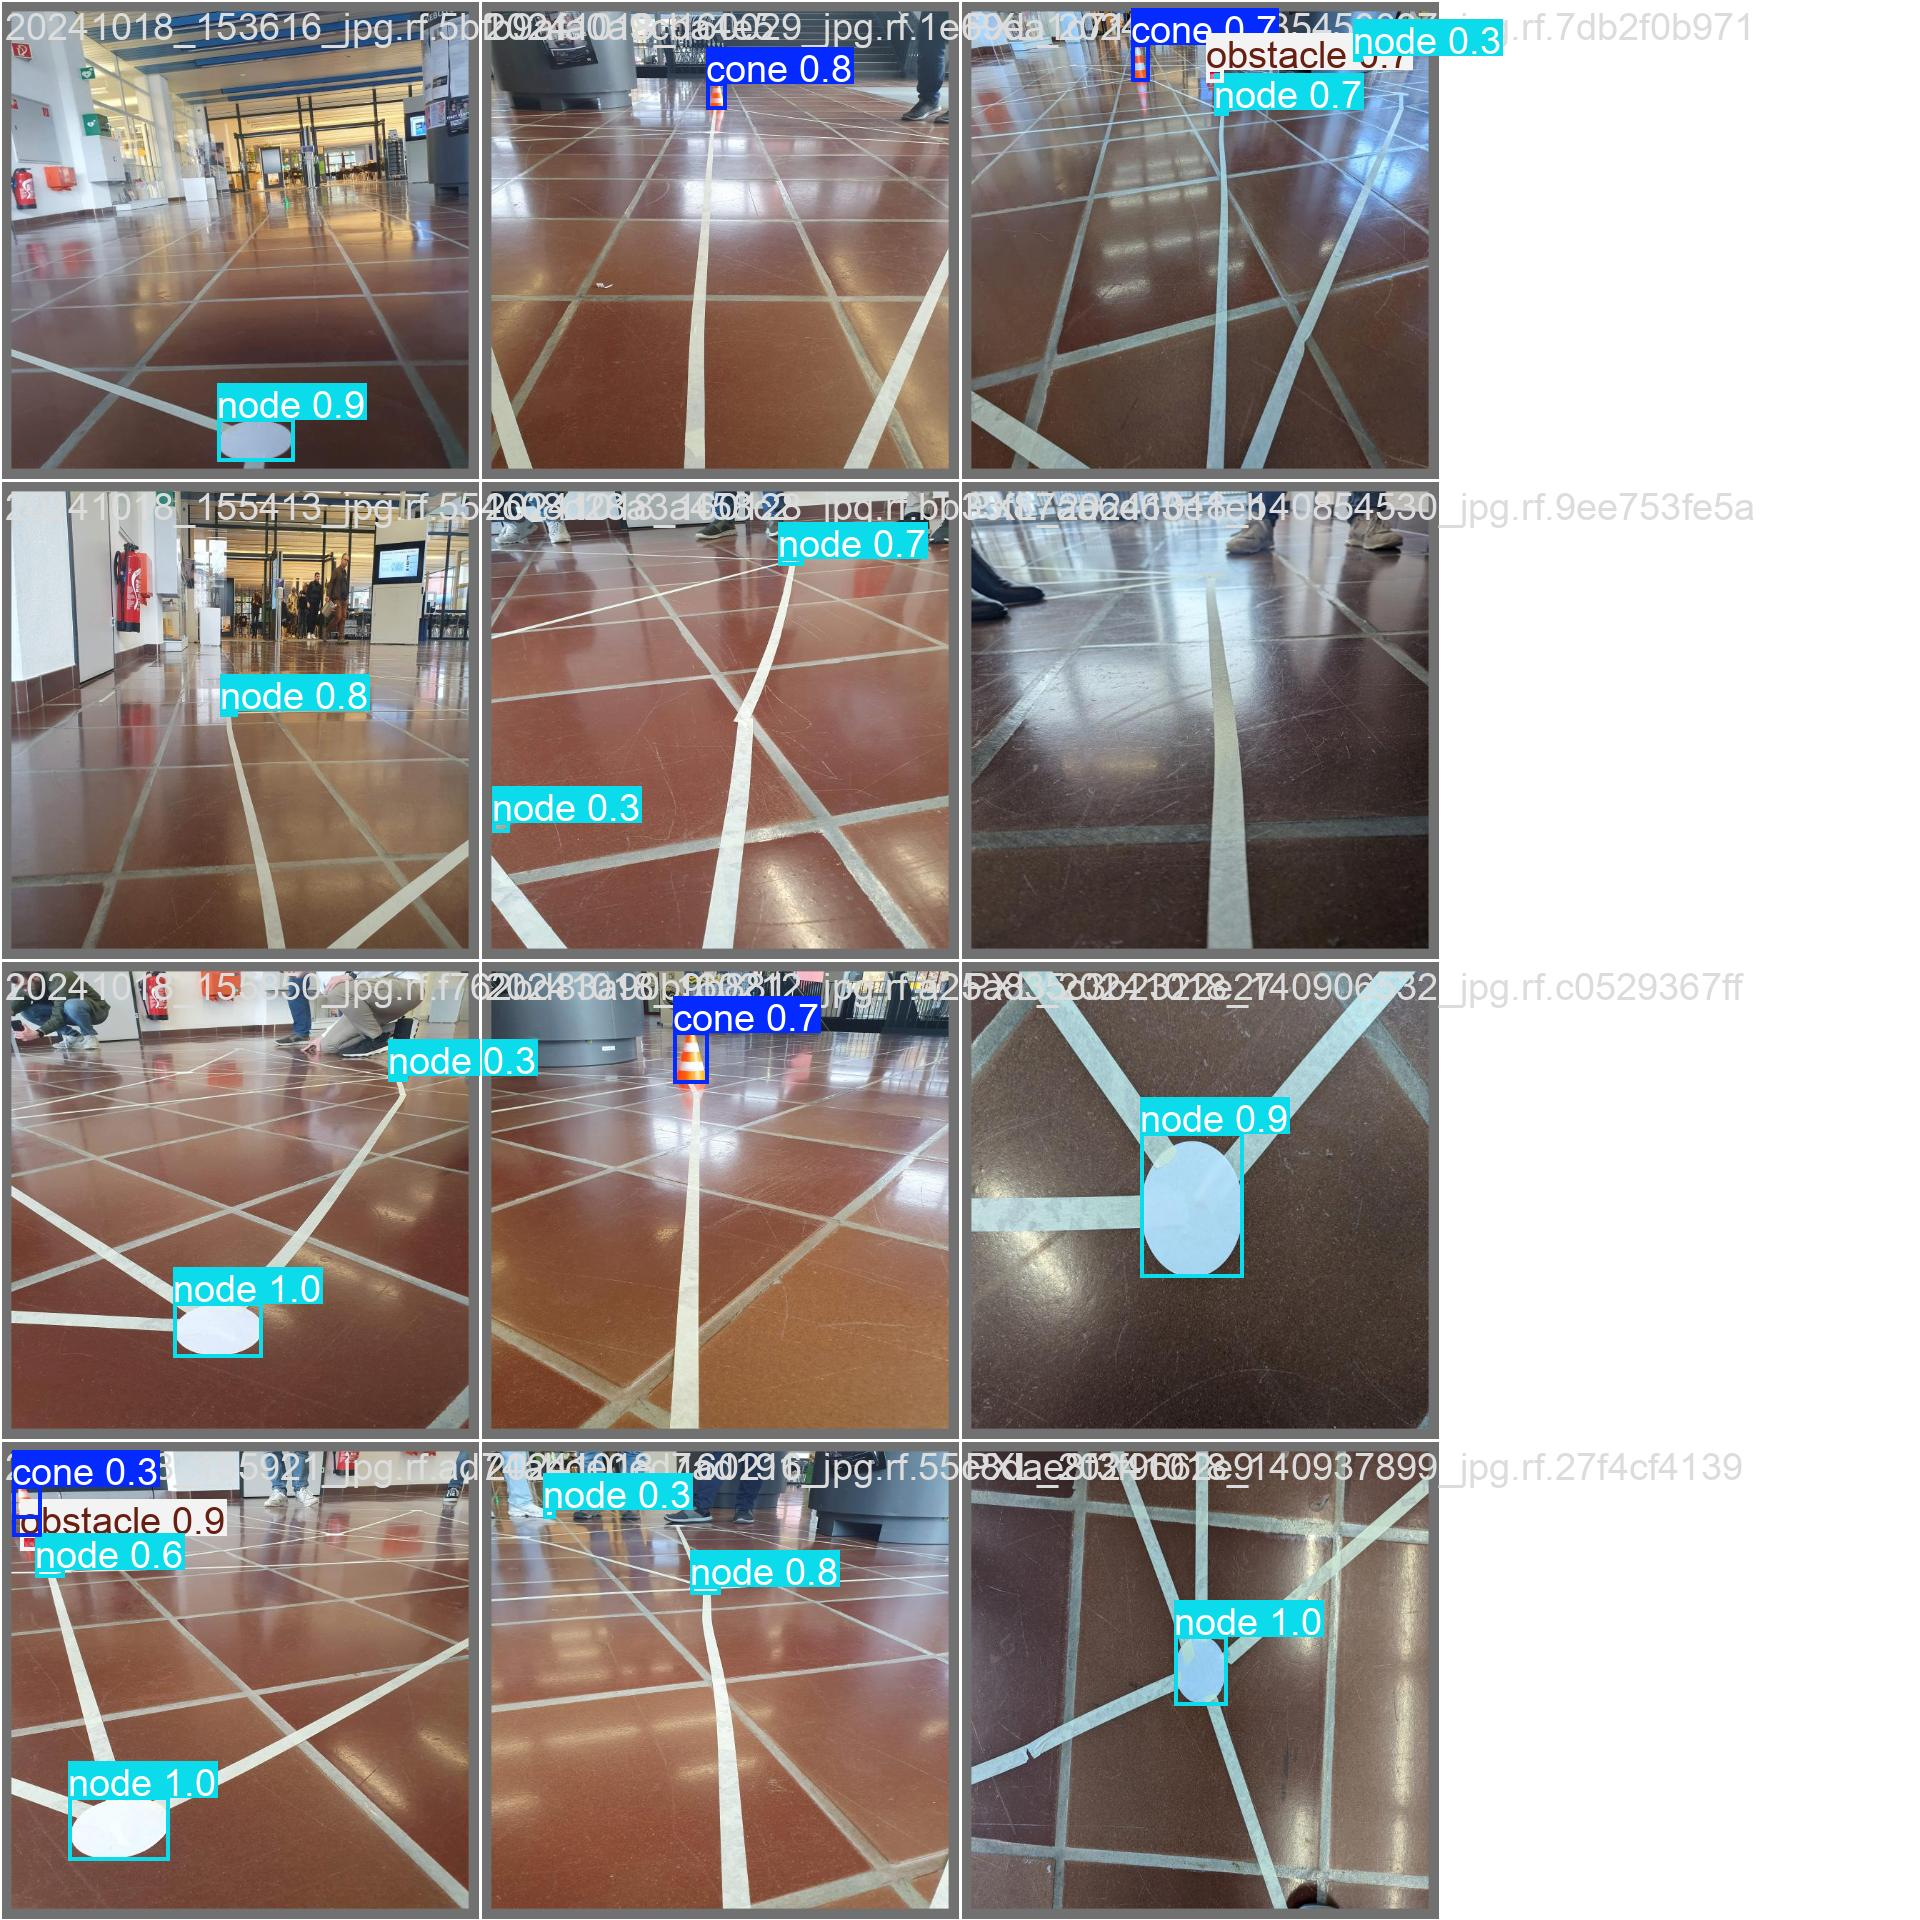
\includegraphics[width=\textwidth -30mm]{assets/informatik-prototyp/yolo/recognized-images.jpeg}
\caption{YOLOv11 Bilderkennung}
\label{fig:img-recognition-yolo}
\end{figure}

-> Yolo kann relativ gut erkennen, vor allem wenn Knoten nicht zu weit weg sind


\textbf{FAST, SIFT}

PLACEHOLDER

\textbf{Objekterkennung mit OpenCV}

PLACEHOLER